

\section{Interactive Analysis}
\label{sec:app_err_analysis}

While our use of \sysname so far relied on automatic selection of counterfactuals, we show in this section how an analyst can benefit from \emph{multiple} counterfactuals per $x$, make use of controlled generation for more advanced analysis, and extract general patterns from individual observations.
Our use case is counterfactual error analysis~\cite{wu2019errudite} of RoBERTa finetuned on \nli (used in \S\ref{subsec:contrast_set}), although the techniques are generally applicable.

There is a known correlation between the label \emph{contradiction} and hypotheses with negation in \nli datasets~\cite{gururangan2018annotation}, which may cause models to fail on non-contradiction negations.
We explore this in Figure~\ref{fig:err_analysis} by generating counterfactual hypotheses for a random \emph{neutral} instance, conditioning only on the original $x$ and the \texttt{negation} \tagstr.
While the first two counterfactuals display this failure mode, there is a surprising inconsistency in model behavior between ``not'' and ``n't''.
We note that manual analysis may not explore these three negation forms, and thus cannot surface this puzzling behavior.


\begin{figure}[t]
\centering
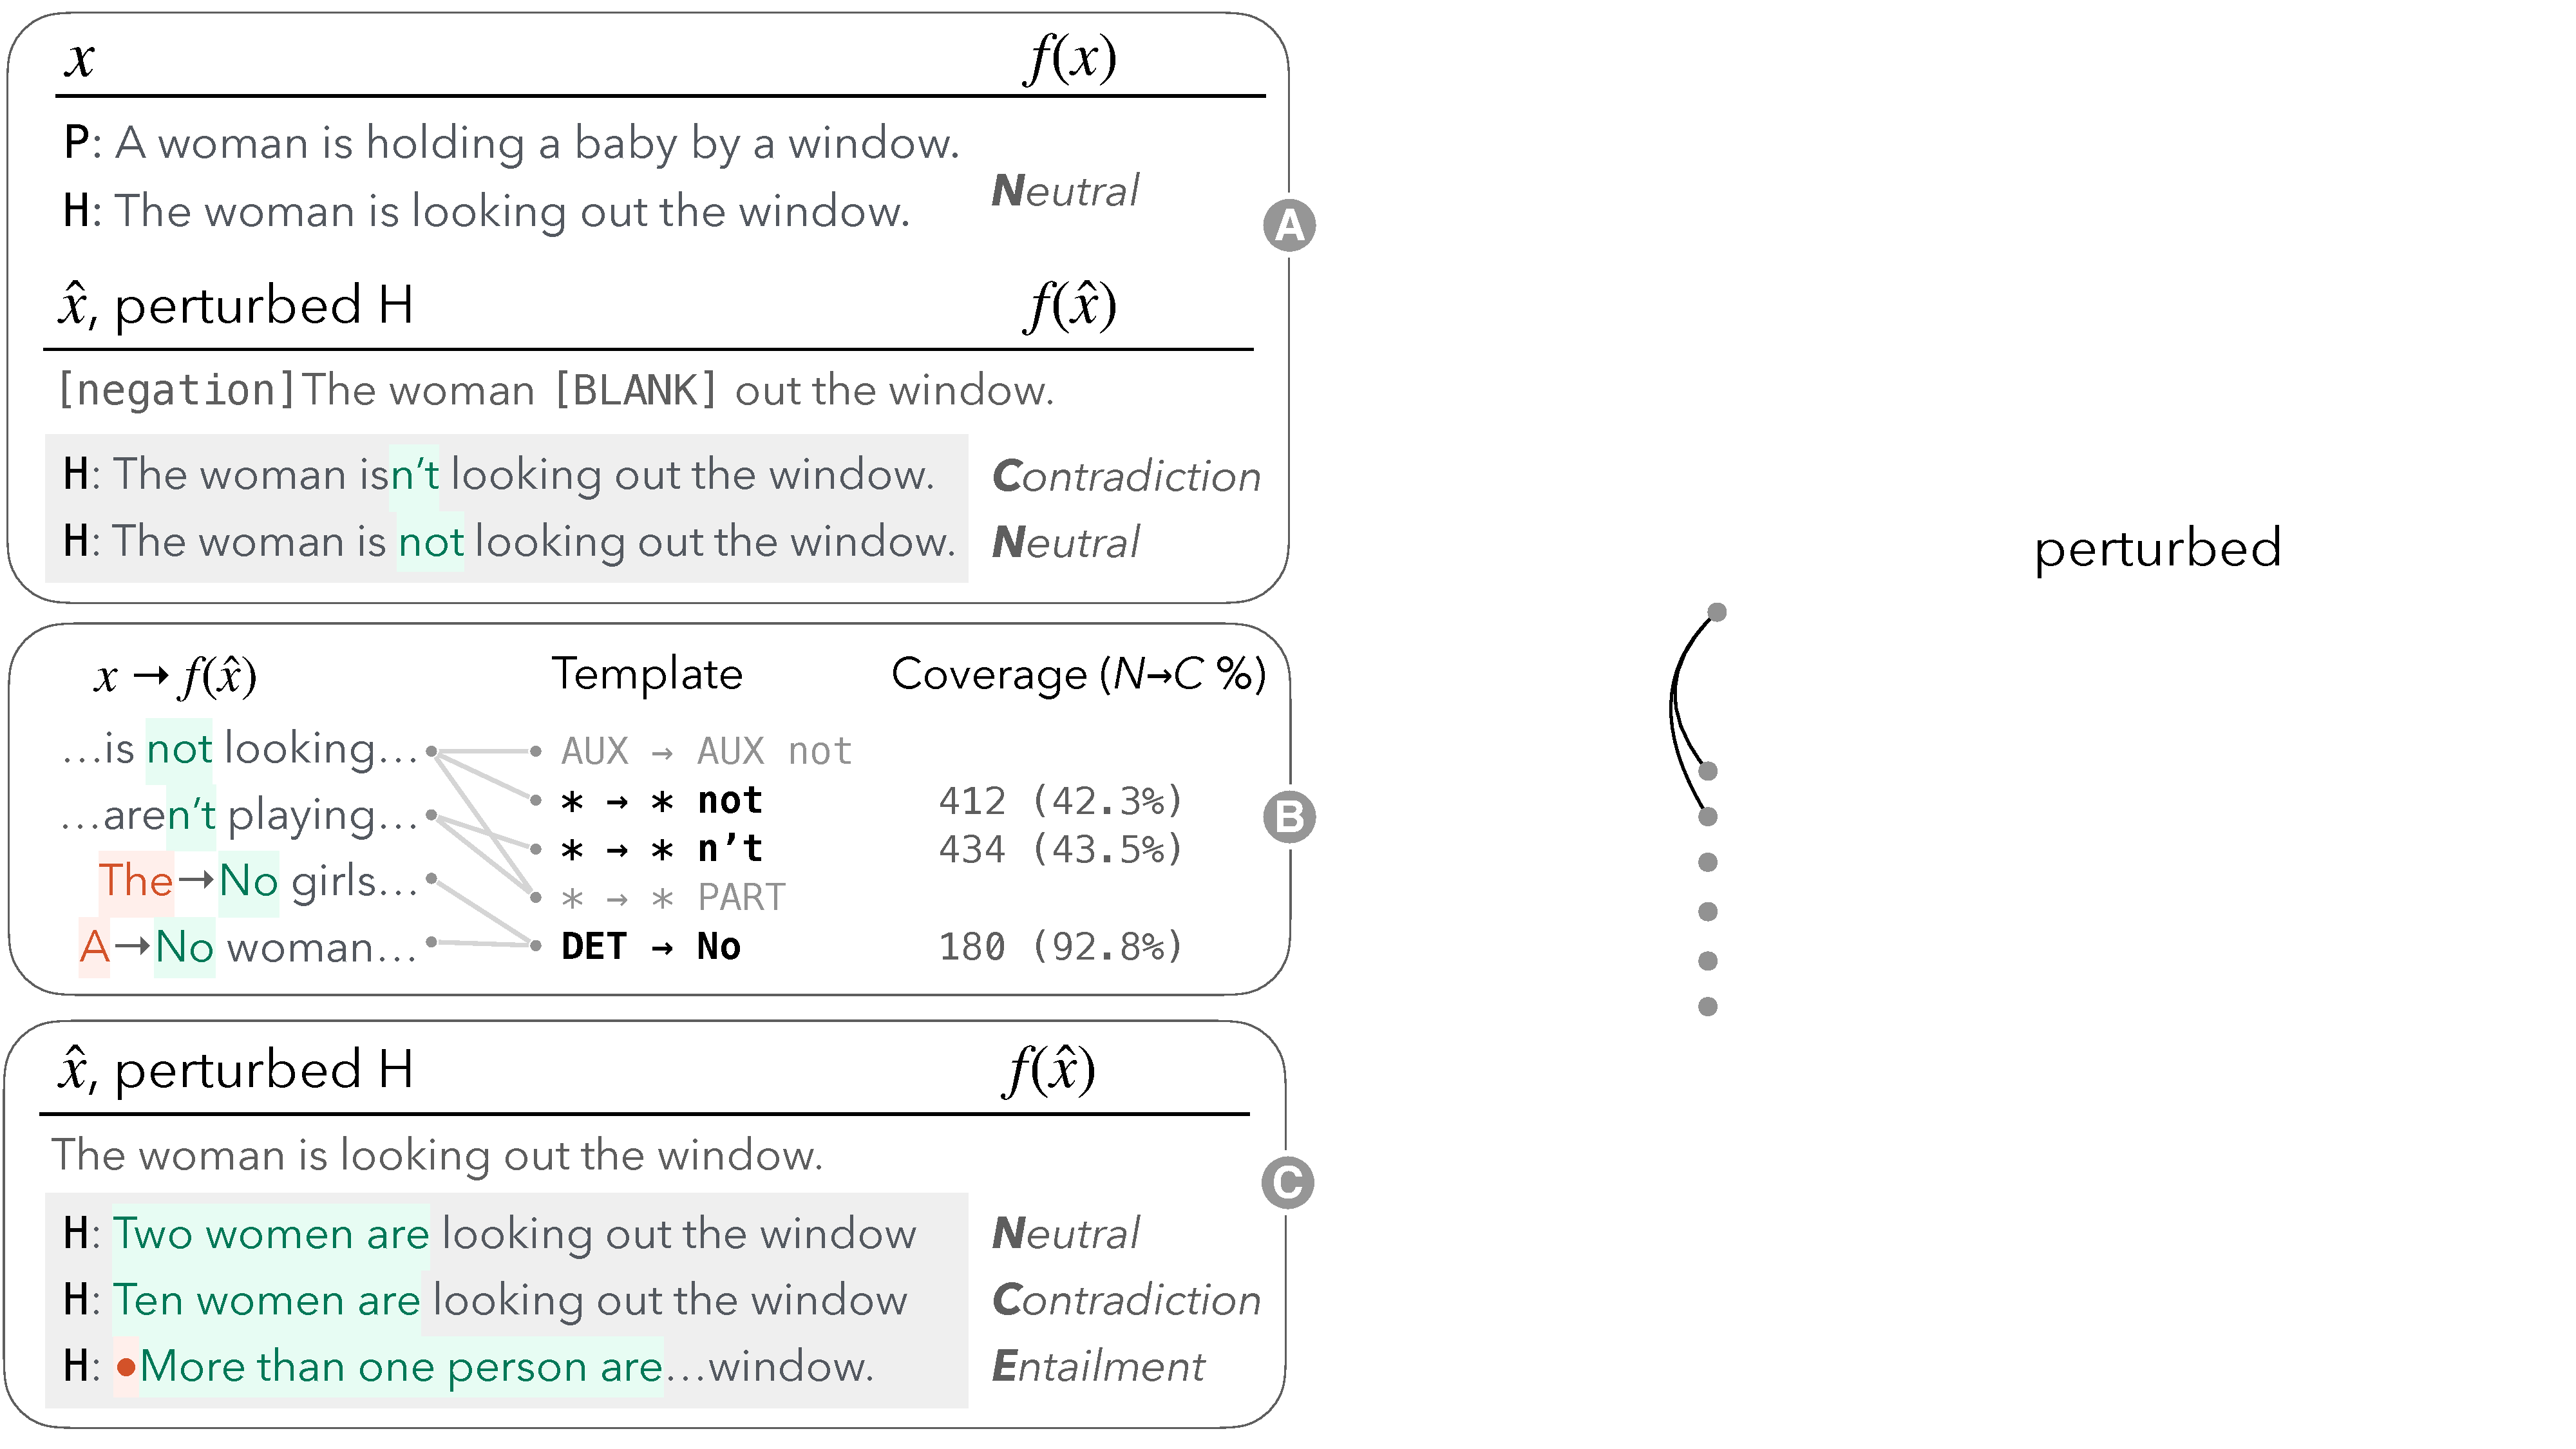
\includegraphics[trim={0 12.5cm 33cm 0cm},clip,width=1\columnwidth]{figures/err_analysis.pdf}
\vspace{-15pt}
\caption{
(A) An \nli case with a \emph{Neutral} prediction (\uline{underlined} $f(\xp)$ are correct).
\sysname generates counterfactual hypotheses conditioned on the \texttt{negation} \tagstr. 
(B) Generalizing perturbations into patterns~\cite{wu2020tempura}. The change \swap{\texttt{DET}}{no} flips $92.8\%$ of predictions from \emph{N}eutral~$\veryshortarrow$~\emph{C}ontradiction.
%(C) Another blank placement that leads to analyses on \emph{quantifiers}.
}
\vspace{-15pt}
\label{fig:err_analysis}
\end{figure}


To verify if the pattern is widespread, we generate counterfactuals with the \texttt{negation} \tagstr for a random set of instances correctly predicted as \emph{neutral} ($n=895$). To generalize individual changes into patterns, we extract frequent \emph{counterfactual templates} with Tempura~\cite{wu2020tempura} (details in Appendix~\ref{appendix:err_analysis_template}), shown in Figure~\ref{fig:err_analysis}B.
The top templates (in bold) show that the model flips its prediction from \emph{neutral} to \emph{contradiction} with roughly the same frequency (${\approx}43\%$) whether the negation word is ``not'' or ``n't'', but flips much more frequently with a different negation pattern where a determiner is replaced with ``no'' ($92.8\%$). While these behaviors may be correct in some instances, they often are not (\eg Figure~\ref{fig:err_analysis}A), and thus would warrant further exploration, and potential mitigation strategies (\eg counterfactual training, \S\ref{sec:app_label}).
Tangentially, the impact of \swap{\texttt{DET}}{no} might lead the analyst to explore the impact of perturbing the \emph{subject} of hypotheses, which we do in Figure~\ref{fig:err_analysis_quantifier} by placing a \texttt{[BLANK]} on the subject rather than using a control code.
This leads to the discovery of unstable and erroneous behaviors regarding \emph{quantifiers}, an analysis that we defer to Appendix~\ref{appendix:err_analysis_quantifier_case}.


\begin{figure}[t]
\centering
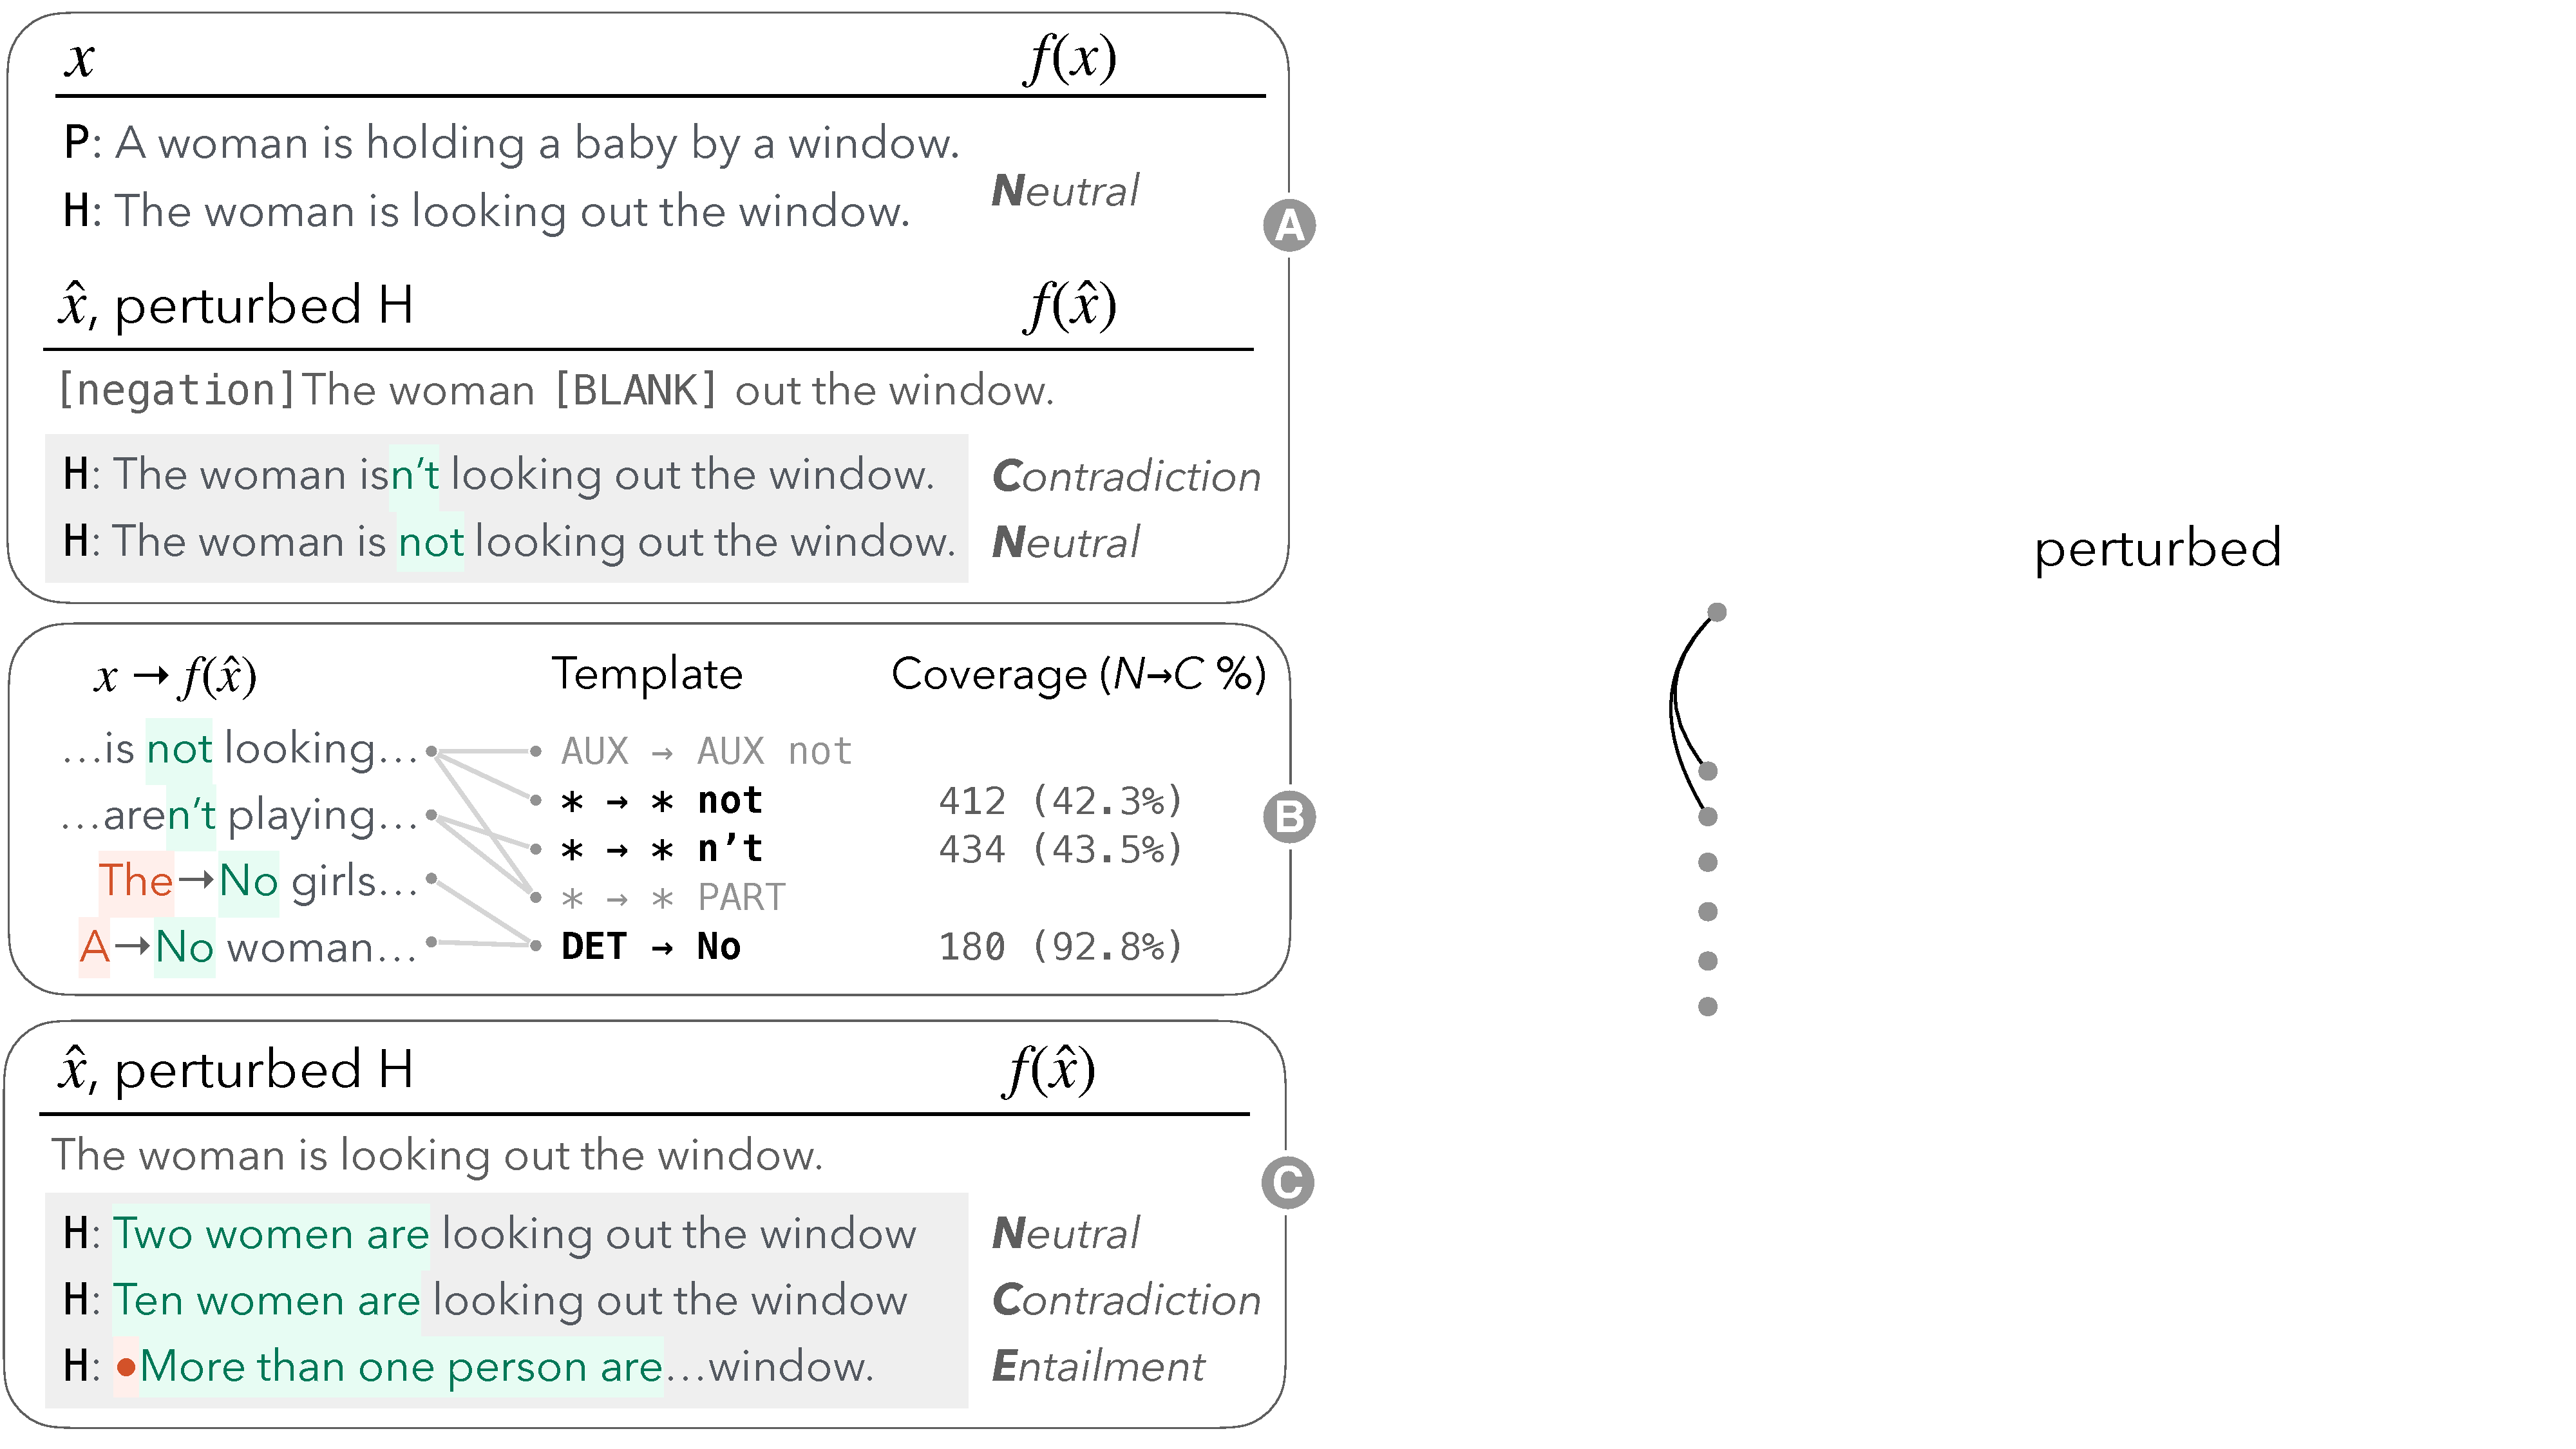
\includegraphics[trim={0.5cm 1.5cm 32.5cm 25.5cm}, clip,width=1\columnwidth]{figures/err_analysis.pdf}
\vspace{-15pt}
\caption{
Perturbing the subject of $x$ in Figure~\ref{fig:err_analysis}A through \texttt{[BLANK]}, resulting in erroneous predictions for different \emph{quantifiers}
(all should be \uline{\emph{Neutral}}). 
}
\vspace{-10pt}
\label{fig:err_analysis_quantifier}
\end{figure}


\paragraph{Discussion.} 
\sysname{} is a powerful tool for interactive analysis.
Generating multiple counterfactuals per instance leads to insights that might be missed by manual analysis, and the controls provided by \tagstrs and \texttt{[BLANK]}s allow for analyses that would be very hard to do manually~\cite{wu2019errudite} or with masked language models (\eg Figure~\ref{fig:err_analysis}B places negations in various parts of sentences, and Figure~\ref{fig:err_analysis_quantifier} replaces spans with other spans of varying lengths). Besides error analysis, an analogous interactive use of \sysname{} may be suitable for test creation~\cite{checklist:acl20} and forms of data augmentation that are more guided than what we presented in \S\ref{sec:app_label}.

% \emph{Verify the hypothesis by generalizing the pattern.}
% Does the observation generalize beyond one instance? 
% We compare different negation patterns on a group of 895 instances that have \emph{neutral} groundtruths and predictions.
% For each $x$, we negate the hypothesis to collect up to 10 counterfactuals (through beam search), and extract \emph{negation templates} from each $\xp$ by abstracting the modified spans into linguistic features (as in Figure~\ref{fig:err_analysis}B).
% Then, we select representative templates that cover various counterfactuals and are as concrete as possible. 
% The method is slightly modified from \citet{wu2020tempura}, and more details are in Appendix~\ref{appendix:err_analysis_template}.
% The top three templates selected (in bold) show interesting contrasts:
% First, counter to Figure~\ref{fig:err_analysis}A, the model is relatively stable on \add{not} and \add{n't} --- they both flip around 43\% \emph{neutral} predictions to \emph{contradiction}, while maintaining others.
% However, the model does respond much more aggressively to \swap{\texttt{DET}}{no}, partially confirming our hypothesis.


% we take a random \emph{neutral} instance in Figure~\ref{fig:err_analysis}A and generate counterfactual hypotheses with \sysname, 

% Previous applications focus on a selected subset of $\xp$, but access to the entire pool is also important.
% we demonstrate that \sysname's ability to generate \emph{multiple} counterfactuals per $x$ is essential for systematic error analysis~\cite{wu2019errudite}.
%Here, the generation is largely driven by human analysts, and the relationship $\relation{\xp}$ can be determined by human domain expertise.

% \emph{Form model behavior hypotheses by inspecting counterfactuals around one instance.}
% \citet{gururangan2018annotation} asserted that negation is correlated with the class label \emph{contradiction}. 
% To verify this, we randomly can select \emph{neutral} instances, and inspect counterfactuals that negate the hypothesis sentence.
% When we apply the \texttt{negation} \tagstr to the hypothesis \emph{H} in Figure~\ref{fig:err_analysis}A, \sysname automatically select different locations of blanks, and produce multiple counterfactuals. 
% Just with a subset of its $\xp$, we notice that the model has some puzzling behavior on negation: 
% While \exinline{is\add{n't}} and \exinline{\swap{The}{No} woman} seem to confirm the overfit to negation, \exinline{is \add{not}} shows a counterexample. 
% We therefore hypothesize that
% \emph{the model has more nuanced responses to different kinds of negation}.


% \emph{Verify the hypothesis by generalizing the pattern.}
% Does the observation generalize beyond one instance? 
% We compare different negation patterns on a group of 895 instances that have \emph{neutral} groundtruths and predictions.
% For each $x$, we negate the hypothesis to collect up to 10 counterfactuals (through beam search), and extract \emph{negation templates} from each $\xp$ by abstracting the modified spans into linguistic features (as in Figure~\ref{fig:err_analysis}B).
% Then, we select representative templates that cover various counterfactuals and are as concrete as possible. 
% The method is slightly modified from \citet{wu2020tempura}, and more details are in Appendix~\ref{appendix:err_analysis_template}.
% The top three templates selected (in bold) show interesting contrasts:
% First, counter to Figure~\ref{fig:err_analysis}A, the model is relatively stable on \add{not} and \add{n't} --- they both flip around 43\% \emph{neutral} predictions to \emph{contradiction}, while maintaining others.
% However, the model does respond much more aggressively to \swap{\texttt{DET}}{no}, partially confirming our hypothesis.



% \emph{Drill-down through interactive blanking.}
% Intrigued by the large impact of \swap{\texttt{DET}}{no}, we decide to explore the importance of the subject more broadly. 
% We explicitly blank the subject as in Figure~\ref{fig:err_analysis_quantifier}, and enumerate through all possible \tagstrs.
% The wild predictions lead us to further hypothesize that the model does not understand quantifiers, which we verify in Appendix~\ref{appendix:err_analysis_quantifier_case}.

% \paragraph{Discussions.}

% \sysname provides unique support for interactive and targeted generation.
% First, by generating multiple counterfactuals, it helps analysts contrast similar perturbations and form hypotheses that might otherwise be missed.
% Analysts rarely check both \swap{is}{is not} and \swap{is}{isn't}, and therefore can overlook potential differences, echoing our observation (\S\ref{sec:app_explain}) that manual counterfactual analysis can be non-exhaustive and misleading.
% Second, \sysname's ability to control the generation (through \tagstrs and blank placements) makes it a powerful tool for interactive and targeted analysis. 
% Such analysis can be hard be achieve with existing masked language models.
% For example, as RoBERTa does not accept any form of controls, we can only obtain a much smaller set of negation counterfactuals by chance.
% Further, with RoBERTa restricted to word substitutions, it cannot produce the examples in Figure~\ref{fig:err_analysis_quantifier}.